\begin{frame}[fragile]
\frametitle{Nested restrict pointers (TLU)}
\begin{minipage}{0.7\textwidth}
\begin{minted}[escapeinside=||,mathescape=true,linenos]{c}
// Scope $\scope{foo}$
int foo(int *restrict *restrict p, int *restrict *restrict q) {
    **p = 10;
    **q = 11;
    return **p; // Optimized to 10 by GCC
}
// Scope $\scope{main}$
int main() {
    int x;
    int* xp = &x;
    foo(&xp, &xp);
}
\end{minted}
\end{minipage}%
\begin{minipage}[t]{0.3\textwidth}
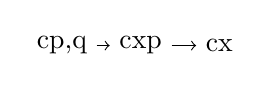
\begin{tikzpicture}
    \node (pq) {\mintinline{c}{p,q}};
    \node[right of = pq] (xp) {\mintinline{c}{xp}};
    \node[right of = xp] (x) {\mintinline{c}{x}};

    \draw[->] (pq) -- (xp);
    \draw[->] (xp) -- (x);
\end{tikzpicture}
\end{minipage}

\begin{itemize}
    \item UB due to a subtle subclause of the standard
\end{itemize}

\end{frame}


% Restrict definition
\begin{frame}
\frametitle{Restrict definition (simplified)}
\begin{itemize}
    % \item A type qualifier for \textbf{pointer types}, \eg \mintinline{c}{int* restrict p;}
    \item A pointer is ``based on'' a restrict pointer if it depends on its value: \\
        \mintinline[mathescape=true]{c}{int x; int* restrict p = &x; int* q = p; // $q$ is based on $p$}  
    \item A \textbf{promise} from the programmer to the compiler that a restrict qualified pointer and pointers ``based on" it will \textbf{not alias} with other pointers during the \textbf{scope} it is alive if:
            \begin{itemize}
                \item The pointer is used to \textbf{access} the object it points to
                \item The object pointed to is \textbf{modified} (by any means)
            \end{itemize}
    \item \colorbox{red!20}{``Modifications of the object pointed to by a restrict pointer are considered to modify} \\ \colorbox{red!20}{the restrict pointer object itself"}
\end{itemize}
\end{frame}




\begin{frame}[fragile]
\frametitle{Nested restrict pointers (TLU)}
\begin{itemize}
    \item What does ``modifications of the object pointed to by a restrict pointer are considered to modify the restrict pointer object itself" mean?
    \item Modifications are represented by the restrict state $\restrictedn$
\end{itemize}

\pause

\begin{figure}[h]
\centering
\begin{minipage}{.5\textwidth}
\begin{minted}[escapeinside=||,mathescape=true]{c}
// Scope $\scope{main}$
{
int x; // $\&x = \Blockvar_x$
int* restrict p = &x; // $\&p = \Blockvar_p$
|\colorbox{red!20}{*p = 10;}| // Modification
}
\end{minted}
\end{minipage}%
\begin{minipage}{.5\textwidth}
\executionannotation
{
    \{$\Blockvar_x \mapsto \colorbox{red!20}{10}$, \\
      \ $\Blockvar_p \mapsto \ptr{(\Blockvar_x, \set{(\Blockvar_p, \scope{main})})}$
    \}
}
{
\begin{tikzpicture}[stack/.style={rectangle split, rectangle split parts=#1, draw, anchor=center, text centered},
    scope/.style={fill=gray!20, anchor=center}]

\node[stack=1, minimum width=4.0cm] (s) {
    \nodepart{one} \{\colorbox{red!20}{$\Blockvar_x \mapsto \restricted{\set{(\Blockvar_p, \scope{main})}}$} \}

};

\node[scope, left=5pt of s.one west]   {\scope{main}};

\end{tikzpicture}
}
\end{minipage}
\end{figure}


\end{frame}

\begin{frame}[fragile]
\frametitle{Nested restrict pointers (TLU)}
\begin{itemize}
    \item What does ``modifications of the object pointed to by a restrict pointer are considered to modify the restrict pointer object itself" mean?
    \item Modifications are represented by the restrict state \colorbox{blue!20}{$\restrictedn$}
\end{itemize}

\begin{figure}[h]
\centering
\begin{minipage}{.5\textwidth}
\begin{minted}[escapeinside=||,mathescape=true]{c}
// Scope $\scope{main}$
{
int x; // $\&x = \Blockvar_x$
int* restrict p = &x; // $\&p = \Blockvar_p$
|\colorbox{red!20}{*p = 10;}| // Modification
}
\end{minted}
\end{minipage}%
\begin{minipage}{.5\textwidth}
\executionannotation
{
    \{$\Blockvar_x \mapsto \colorbox{red!20}{10}$, \\
        \ $\Blockvar_p \mapsto \ptr{(\Blockvar_x, \set{(\Blockvar_p, \scope{main})})}$
    \}
}
{
\begin{tikzpicture}[stack/.style={rectangle split, rectangle split parts=#1, draw, anchor=center, text centered},
    scope/.style={fill=gray!20, anchor=center}]

\node[stack=1, minimum width=4.0cm] (s) {
    \nodepart[align=left]{one} \{\colorbox{red!20}{$\Blockvar_x \mapsto \restricted{\set{(\Blockvar_p, \scope{main})}}$}, \\
                    \ \colorbox{blue!20}{$\Blockvar_p \mapsto \restricted{\emptyset} $} \}

};

\node[scope, left=5pt of s.one west]   {\scope{main}};

\end{tikzpicture}
}
\end{minipage}
\end{figure}


\end{frame}



\begin{frame}[fragile]
\frametitle{Nested restrict pointers (TLU)}
\begin{minted}[escapeinside=||,mathescape=true]{c}
// Scope $\scope{foo}$
int foo(int *restrict *restrict p, int *restrict *restrict q) {
    *|\colorbox{red!20}{*p}| = 10;
    **q = 11;
    return **p;
}
\end{minted}

\vspace*{-2cm}

\begin{figure}[!h]
\begin{minipage}[t]{.36\textwidth}
\begin{minted}[escapeinside=||,mathescape=true]{c}
// Scope $\scope{main}$
int main() {
    int x;
    int* xp = &x;
    foo(&xp, &xp);
}
\end{minted}
\end{minipage}%
\begin{minipage}{.64\textwidth}

\executionannotation
{
\{ $\Blockvar_x \mapsto \vundef$, \\
    \ $\Blockvar_{xp} \mapsto \ptr{(\Blockvar_x, \emptyset)}$, \\
    \ $\Blockvar_p \mapsto \ptr{(\Blockvar_{xp}, \set{(\Blockvar_p, \scope{foo})})}$, \\
    \ $\Blockvar_q \mapsto \ptr{(\Blockvar_{xp}, \set{(\Blockvar_q, \scope{foo})})}$ \}
}
{
    \begin{tikzpicture}[stack/.style={rectangle split, rectangle split parts=#1, draw, anchor=center, text centered},
        scope/.style={fill=gray!20, anchor=center}]
    \node[stack=2, minimum width=4.0cm] (s) {
    \nodepart{one} \{\colorbox{red!20}{..., $\Blockvar_{xp} \mapsto \onlyread{\set{(\Blockvar_p, \scope{foo})}}$}\}
    \nodepart{two} $\emptyset$
    };
    \node[scope, left=5pt of s.one west]   {\scope{foo}};
    \node[scope, left=5pt of s.two west]   {\scope{main}};
    \end{tikzpicture}   
}

\end{minipage}
\end{figure}


\end{frame}



\begin{frame}[fragile]
\frametitle{Nested restrict pointers (TLU)}
\begin{minted}[escapeinside=||,mathescape=true]{c}
// Scope $\scope{foo}$
int foo(int *restrict *restrict p, int *restrict *restrict q) {
    |\colorbox{red!20}{**p}| = 10;
    **q = 11;
    return **p;
}
\end{minted}

\vspace*{-2cm}

\begin{figure}[!h]
\begin{minipage}[t]{.36\textwidth}
\begin{minted}[escapeinside=||,mathescape=true]{c}
// Scope $\scope{main}$
int main() {
    int x;
    int* xp = &x;
    foo(&xp, &xp);
}
\end{minted}
\end{minipage}%
\begin{minipage}{.64\textwidth}

\executionannotation
{
\{ $\Blockvar_x \mapsto \vundef$, \\
    \ $\Blockvar_{xp} \mapsto \ptr{(\Blockvar_x, \emptyset)}$, \\
    \ $\Blockvar_p \mapsto \ptr{(\Blockvar_{xp}, \set{(\Blockvar_p, \scope{foo})})}$, \\
    \ $\Blockvar_q \mapsto \ptr{(\Blockvar_{xp}, \set{(\Blockvar_q, \scope{foo})})}$ \}
}
{
    \begin{tikzpicture}[stack/.style={rectangle split, rectangle split parts=#1, draw, anchor=center, text centered},
        scope/.style={fill=gray!20, anchor=center}]
    \node[stack=2, minimum width=4.0cm] (s) {
    \nodepart[align=left]{one} \{$..., \Blockvar_{xp} \mapsto \onlyread{\set{(\Blockvar_p, \scope{foo})}}$, \\
                     \ \colorbox{red!20}{$\Blockvar_x \mapsto \restricted{\set{(\Blockvar_{xp}, \scope{foo})}}$}\}
    \nodepart{two} $\emptyset$
    };
    \node[scope, left=5pt of s.one west]   {\scope{foo}};
    \node[scope, left=5pt of s.two west]   {\scope{main}};
    \end{tikzpicture}   
}

\end{minipage}
\end{figure}

\end{frame}


\begin{frame}[fragile]
\frametitle{Nested restrict pointers (TLU)}

\begin{itemize}
    \item We now need to change the restrict state of $\Blockvar_{xp}$ to $\restrictedn$
    \item The only $\restrictedn$ state joinable with the current state is \colorbox{blue!20}{$\restricted{\set{(\Blockvar_p, \scope{foo})}}$}
    \item Problem: \textbf{not enough information} to produce this state, \ie the semantics did a store through $\ptr{(\Blockvar_x, \set{(\Blockvar_{xp}, \scope{foo})})}$
\end{itemize}

\leavevmode \\

\begin{tikzpicture}[stack/.style={rectangle split, rectangle split parts=#1, draw, anchor=center, text centered},
    scope/.style={fill=gray!20, anchor=center}]
\node[stack=2, minimum width=4.0cm] (s) {
\nodepart[align=left]{one} \{..., $\Blockvar_{xp} \mapsto \onlyread{\set{(\Blockvar_p, \scope{foo})}}$, \\
                 \ $\Blockvar_x \mapsto \restricted{\set{(\Blockvar_{xp}, \scope{foo})}}$\}
\nodepart{two} $\emptyset$
};
\node[scope, left=5pt of s.one west]   {\scope{foo}};
\node[scope, left=5pt of s.two west]   {\scope{main}};
\end{tikzpicture}

\end{frame}


\begin{frame}
\frametitle{Nested restrict pointers (TLU)}

\begin{itemize}
    \item Idea: pointer value as a \textbf{tree} structure, to track how bases themselves are derived!
    \item $\ptr{(\Blockvar_x, \set{((\Blockvar_{xp}, \set{((\Blockvar_p, \emptyset), \scope{foo})}), \scope{foo})})}$ \\~\\
    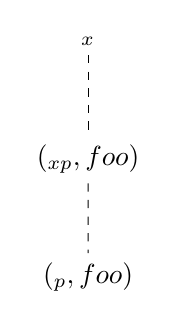
\begin{tikzpicture}[sibling distance=25mm,      edge from parent/.style={draw, dashed},
        every edge/.append style={->}    ]
    \node (root) {$\Blockvar_x$}
        child {node {$(\Blockvar_{xp}, \scope{foo})$}
        child {node {$(\Blockvar_p, \scope{foo})$}}
        };
    
    \end{tikzpicture}

\end{itemize}
    
\end{frame}



\begin{frame}[fragile]
\frametitle{Nested restrict pointers (TLU)}
\begin{minted}[escapeinside=||,mathescape=true]{c}
// Scope $\scope{foo}$
int foo(int *restrict *restrict p, int *restrict *restrict q) {
    |\colorbox{red!20}{**p}| = 10;
    **q = 11;
    return **p;
}
\end{minted}

\vspace*{-2cm}

\begin{figure}[!h]
\begin{minipage}[t]{.3\textwidth}
\begin{minted}[escapeinside=||,mathescape=true]{c}
// Scope $\scope{main}$
int main() {
    int x;
    int* xp = &x;
    foo(&xp, &xp);
}
\end{minted}
\end{minipage}%
\begin{minipage}{.7\textwidth}

\executionannotation
{
\{ $\Blockvar_x \mapsto \vundef$, \\
    \ $\Blockvar_{xp} \mapsto \ptr{(\Blockvar_x, \emptyset)}$, \\
    \ $\Blockvar_p \mapsto \ptr{(\Blockvar_{xp}, \set{((\Blockvar_p, \emptyset), \scope{foo})})}$, \\
    \ $\Blockvar_q \mapsto \ptr{(\Blockvar_{xp}, \set{((\Blockvar_q, \emptyset), \scope{foo})})}$ \}
}
{
    \begin{tikzpicture}[stack/.style={rectangle split, rectangle split parts=#1, draw, anchor=center, text centered},
        scope/.style={fill=gray!20, anchor=center}]
    \node[stack=2, minimum width=4.0cm] (s) {
    \nodepart[align=left]{one} \{..., \colorbox{blue!20}{$\Blockvar_{xp} \mapsto \restricted{\set{((\Blockvar_p, \emptyset), \scope{foo})}}$}, \\
                        \ \colorbox{red!20}{$\Blockvar_x \mapsto \restricted{\set{((\Blockvar_{xp}, \set{((\Blockvar_p, \emptyset), \scope{foo})}), \scope{foo})}}$}\}
    \nodepart{two} $\emptyset$
    };
    \node[scope, left=5pt of s.one west]   {\scope{foo}};
    \node[scope, left=5pt of s.two west]   {\scope{main}};
    \end{tikzpicture}   
}

\end{minipage}
\end{figure}

\end{frame}



\begin{frame}[fragile]
\frametitle{Nested restrict pointers (TLU)}
\begin{minted}[escapeinside=||,mathescape=true]{c}
// Scope $\scope{foo}$
int foo(int *restrict *restrict p, int *restrict *restrict q) {
    **p = 10;
    *|\colorbox{red!20}{*q}| = 11;
    return **p;
}
\end{minted}

\vspace*{-2cm}

\begin{figure}[!h]
\begin{minipage}[t]{.3\textwidth}
\begin{minted}[escapeinside=||,mathescape=true]{c}
// Scope $\scope{main}$
int main() {
    int x;
    int* xp = &x;
    foo(&xp, &xp);
}
\end{minted}
\end{minipage}%
\begin{minipage}{.7\textwidth}

\executionannotation
{
\{ $\Blockvar_x \mapsto \vundef$, \\
    \ $\Blockvar_{xp} \mapsto \ptr{(\Blockvar_x, \emptyset)}$, \\
    \ $\Blockvar_p \mapsto \ptr{(\Blockvar_{xp}, \set{((\Blockvar_p, \emptyset), \scope{foo})})}$, \\
    \ $\Blockvar_q \mapsto \ptr{(\Blockvar_{xp}, \set{((\Blockvar_q, \emptyset), \scope{foo})})}$ \}
}
{
    \begin{tikzpicture}[stack/.style={rectangle split, rectangle split parts=#1, draw, anchor=center, text centered},
        scope/.style={fill=gray!20, anchor=center}]
    \node[stack=2, minimum width=4.0cm] (s) {
    \nodepart[align=left]{one} \{..., \colorbox{blue!20}{$\Blockvar_{xp} \mapsto \restricted{\set{((\Blockvar_p, \emptyset), \scope{foo})}}$}, \\
                        \ \colorbox{red!20}{$\Blockvar_x \mapsto \restricted{\set{((\Blockvar_{xp}, \set{((\Blockvar_p, \emptyset), \scope{foo})}), \scope{foo})}}$}\}
    \nodepart{two} $\emptyset$
    };
    \node[scope, left=5pt of s.one west]   {\scope{foo}};
    \node[scope, left=5pt of s.two west]   {\scope{main}};
    \end{tikzpicture}   
}

\end{minipage}
\end{figure}

\end{frame}



\begin{frame}[fragile]
\frametitle{Nested restrict pointers (TLU)}
\begin{minted}[escapeinside=||,mathescape=true]{c}
// Scope $\scope{foo}$
int foo(int *restrict *restrict p, int *restrict *restrict q) {
    **p = 10;
    *|\colorbox{red!20}{*q}| = 11;
    return **p;
}
\end{minted}

\vspace*{-2cm}

\begin{figure}[!h]
\begin{minipage}[t]{.3\textwidth}
\begin{minted}[escapeinside=||,mathescape=true]{c}
// Scope $\scope{main}$
int main() {
    int x;
    int* xp = &x;
    foo(&xp, &xp);
}
\end{minted}
\end{minipage}%
\begin{minipage}{.7\textwidth}
\colorbox{red!20}{$\onlyread{\set{((\Blockvar_\text{\textcolor{blue}{$q$}}, \emptyset), \scope{foo})}} \joinsym  \restricted{\set{((\Blockvar_\text{\textcolor{blue}{$p$}}, \emptyset), \scope{foo})}} = ...$} \\

\executionannotation
{
\{ ..., \\
    \ $\Blockvar_q \mapsto \ptr{(\Blockvar_{xp}, \set{((\Blockvar_q, \emptyset), \scope{foo})})}$ \}
}
{
    \begin{tikzpicture}[stack/.style={rectangle split, rectangle split parts=#1, draw, anchor=center, text centered},
        scope/.style={fill=gray!20, anchor=center}]
    \node[stack=2, minimum width=4.0cm] (s) {
    \nodepart[align=left]{one} \{..., \colorbox{red!20}{$\Blockvar_{xp}$} $\mapsto \restricted{\set{((\Blockvar_p, \emptyset), \scope{foo})}}$, \\
                        \ $\Blockvar_x \mapsto \restricted{\set{((\Blockvar_{xp}, \set{((\Blockvar_p, \emptyset), \scope{foo})}), \scope{foo})}}$\}
    \nodepart{two} $\emptyset$
    };
    \node[scope, left=5pt of s.one west]   {\scope{foo}};
    \node[scope, left=5pt of s.two west]   {\scope{main}};
    \end{tikzpicture}   
}

\end{minipage}
\end{figure}

\end{frame}






\begin{frame}[fragile]
\frametitle{Nested restrict pointers (TLU)}
\centering
\colorbox{red!20}{$\onlyread{\set{((\Blockvar_\text{\textcolor{blue}{$q$}}, \emptyset), \scope{foo})}} \joinsym  \restricted{\set{((\Blockvar_\text{\textcolor{blue}{$p$}}, \emptyset), \scope{foo})}} = \rsub$} \\

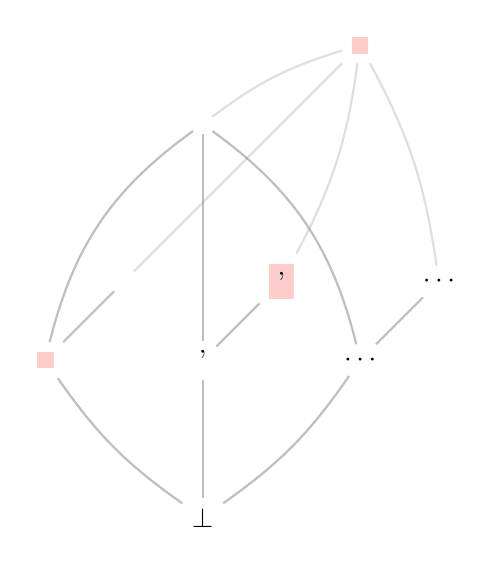
\begin{tikzpicture}
    \node (ub)     at (7,5) {\colorbox{red!20}{\rsub}};
    \node (un)     at (5,4) {\unresabbr};
    \node (rsbs)   at (4,2) {\resabbr{\Basesvar}};
    \node (rsbs')  at (6,2) {\colorbox{red!20}{\resabbr{\Basesvar'}}};
    \node (rsbs'') at (8,2) {$\cdots$};
    \node (orbs)   at (3,1) {\colorbox{red!20}{\orabbr{\Basesvar}}};
    \node (orbs')  at (5,1) {\orabbr{\Basesvar'}};
    \node (orbs'') at (7,1) {$\cdots$};
    \node (bot)    at (5,-1) {$\bot$};

    \path[thick, black, opacity=0.25]
    (bot) edge[bend left=10] node {} (orbs)
    (bot) edge node {} (orbs')
    (bot) edge[bend right=10] node {} (orbs'')
    
    (orbs) edge node {} (rsbs) 
    (orbs') edge node {} (rsbs')
    (orbs'') edge node {} (rsbs'')  
    
    (orbs) edge[bend left=20] node {} (un)
    (orbs') edge node {} (un)
    (orbs'') edge[bend right=20] node {} (un)

    (rsbs) edge[gray] node {} (ub)
    (rsbs') edge[bend right=10, gray] node {} (ub)
    (rsbs'') edge[bend right=10, gray] node {} (ub)

    (un) edge[bend left=10, gray] node {} (ub);
\end{tikzpicture}

\end{frame}


\begin{frame}[fragile]
\frametitle{Nested restrict pointers (TLU)}
\begin{itemize}
    \item Implemented a subtle subclause of the standard (in line with the GCC interpretation)
    \begin{itemize}    
        \item Updated pointer values to a \textbf{tree-like structure} to track how bases themselves are derived
    \end{itemize}
    \item Achieved our goal of giving undefined behavior \smiley{}
\end{itemize}

\end{frame}
